\part{Keypoint Descriptor}\label{part:SIFT descriptor}

在计算机视觉中,为了进行图像处理、目标检测、图像匹配等任务,需要从图像中提取出能够代表图像内容的特征。关键点描述就是这些特征之一,它能够描述图像中的局部特征,通常具有不变性、区分性和可重复性等优良性质,因此在图像匹配和目标识别等任务中被广泛应用。

对于某个关键点,其描述子可以看作是对该点周围像素的一种统计特征表达,它可以用于描述该点的形状、颜色、纹理等信息。在构建关键点描述子时,需要保证其具有一定的不变性,即对于图像的旋转、缩放、平移、光照等变换具有一定的容忍度,这样才能在实际应用中获得更好的效果。因此,\sift 算法采用了一些特殊的技巧来确保描述子的不变性,如使用\DoG 金字塔来实现尺度不变性,使用主方向来实现旋转不变性等。前面部分介绍了如何构建\DoG 金字塔并从中提取关键点,这一部分介绍主方向分配,以及构建具有旋转不变性的关键点描述子。

\section{主方向分配}

在\sift 算法中,\emph{主方向}被定义为是指关键点周围像素的梯度方向直方图中的最大峰值所对应的方向。在找到这个主方向之后,通过对关键点周围的图像区域进行旋转的方式,将该主方向变换到统一的标准方向。该过程的具体步骤如下:
\begin{enumerate}
    \item 计算梯度幅值和方向:首先,以每个\sift 特征关键点为中心提取出$16\times 16$的局部图像块,然后计算其中每个像素的梯度幅值和方向。这可以通过对图像进行梯度运算来实现。通常使用Sobel算子或\lpl 算子来计算图像的梯度。对于像素点$(x,y)$,其梯度的幅值和方向分别为:
    \begin{align}
        m(x, y)&=\sqrt{g_x^2(x, y) + g_y^2(x, y)}\\
        \theta (x, y)&=\arctan \frac{g_y(x, y)}{g_x(x, y)}
        \label{equ: compute gradient}
    \end{align}
    其中,$g_x(x,y)$和$g_y(x,y)$分别表示像素点$(x,y)$处的水平和垂直方向梯度。需要注意的是,在计算梯度方向时,可以将其划分为8个方向(即0度、45度、90度、135度、180度、225度、270度、315度)。
    \item 构建方向直方图:接下来,需要将局部图像块的每个像素的梯度按方向方向分配到8个区间中,统计每个方向区间内的梯度幅值,最后形成一个长度为8的方向直方图。具体来说,对于像素点$(x,y)$,可以根据其梯度方向$\theta(x,y)$将其梯度幅值$m(x,y)$分配到相应的方向区间中。如果$\theta(x,y)$位于第$i$个方向区间内,则该区间的计数器$bin_i$需要增加$m(x,y)$的值。这样,就可以得到一个长度为8的方向直方图:
    \begin{equation*}
        H = \left[bin_1, bin_2, \ldots, bin_8\right]
    \end{equation*}
    \item 寻找主方向:在得到关键点周围的方向直方图后,需要在其中寻找主方向。通常采用最大值法来确定主方向,即在方向直方图中找到最大的那个值,并将其对应的方向作为主方向。同时,可以考虑一些容错机制,例如将大于最大值一半的值也视为主方向,以确保算法的稳定性。
\end{enumerate}

\section{特征描述子}

经过主方向分配后,各幅图像对应特征子周围像素之间的旋转角度不确定性得以消除,所以到目前为止\sift 特征已经解决了尺度问题、旋转问题。对于光照变化,如果直接用\sift 关键点周围的像素直接做比较是明显不合理的,因此\sift 进一步提出了一种更为鲁棒的描述子,即用一个128维向量为关键点进行特征编码,而编码过程考虑的是关键点周围像素的梯度赋值和方向。具体实现过程如下:
\begin{enumerate}
    \item 旋转每个\sift 关键点周围像素,使其主方向能与指定的标准方向对齐,并重新提取以每个\sift 特征关键点为中心的$16\times 16$的局部图像块;
    \item 计算局部图像块每个像素上的梯度幅值与方向。同时按照到中心点的距离对梯度幅值进行高斯加权,高斯函数的标准差按经验一般取$\sigma_w=1.5\times 16$;
    \item 将$16\times 16$的局部图像块再划分为16个$4\times 4$的子块,然后在每个子块中统计一个长度为8的梯度方向直方图,每一个方向的权重为上一步高斯加权后的梯度幅值;
    \item 将这16个长度为8的梯度方向直方图拼成一个128维向量,这个高维向量经过归一化就获得了\sift 特征描述子,它对线性光照变化具有鲁棒性。
\end{enumerate}


\begin{figure}[H]
    \centering
    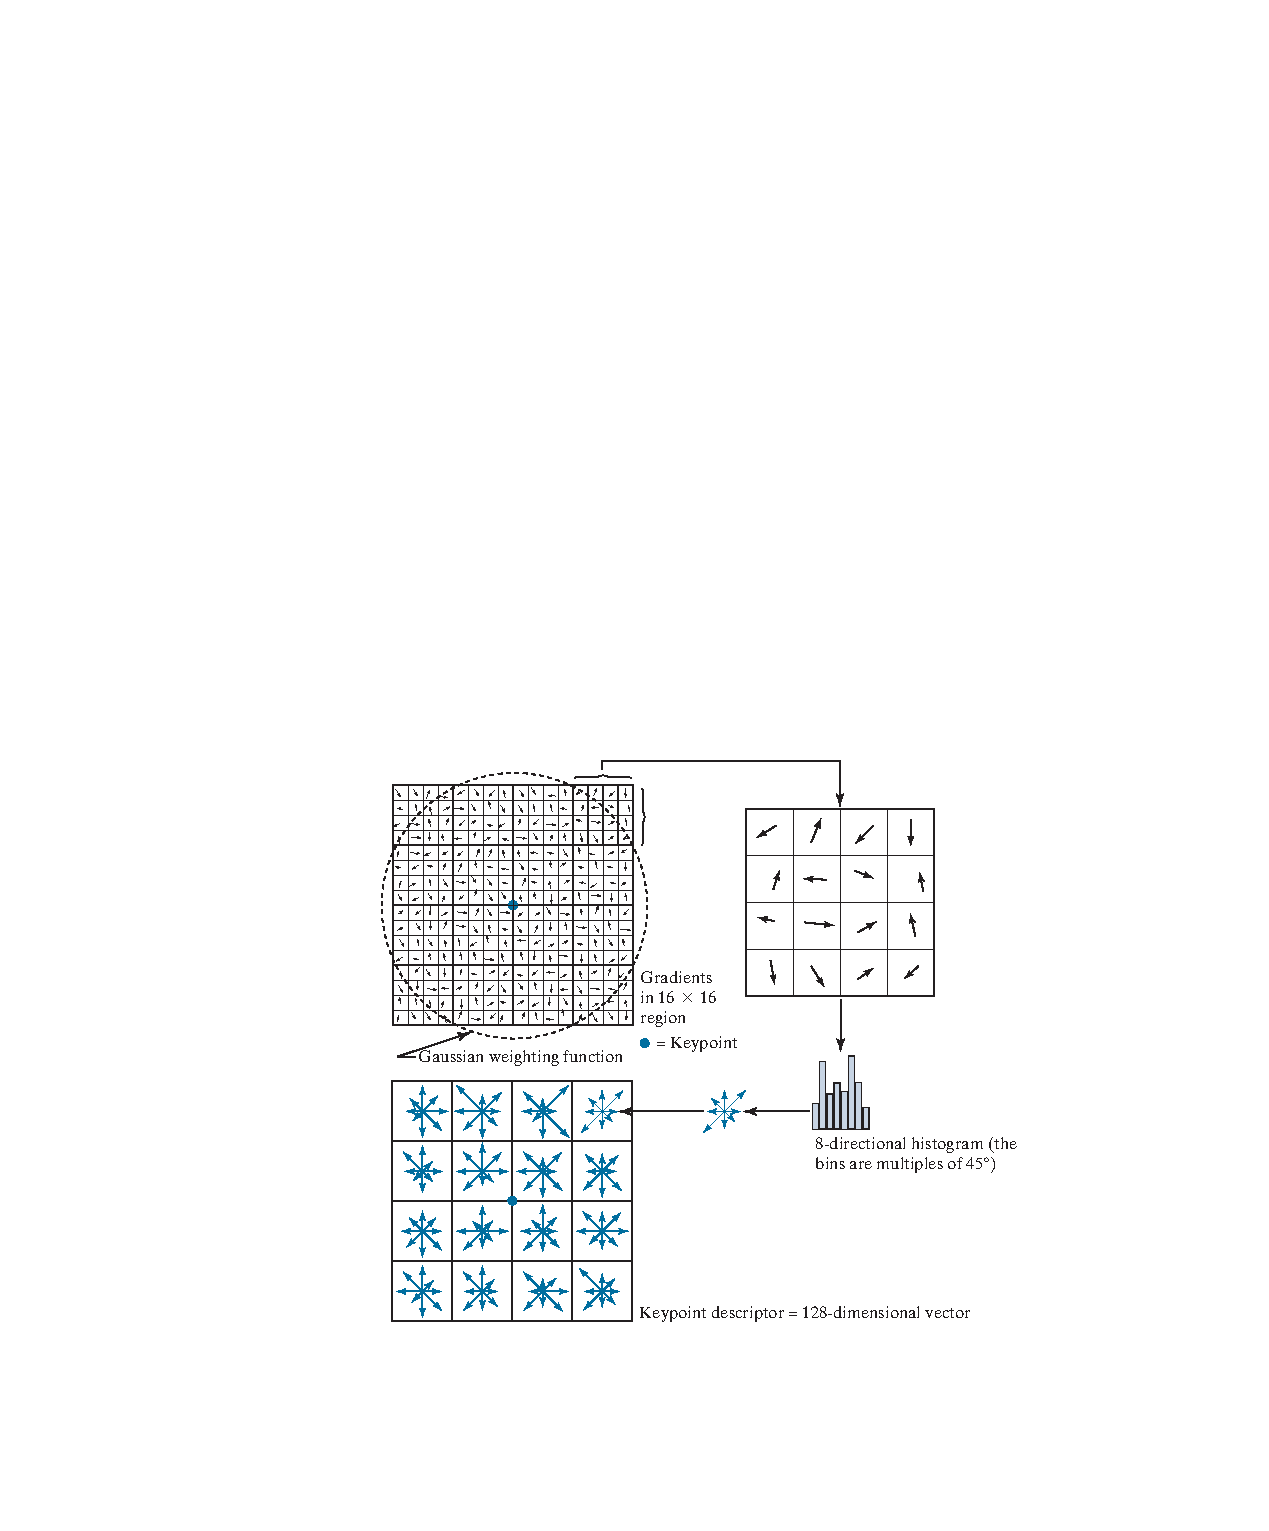
\includegraphics[width=.8\textwidth]{fig/Keypoint descriptor.pdf}
    \caption{\sift 特征描述子}
\end{figure}

\begin{remark}
    对比确定主方向的过程,同样是构建梯度方向的直方图,但在特征描述子当中是需要对16个子块分别构建,并且梯度幅值还被进行了高斯加权。划分子块的方式可以保留更精细的局部细节。
\end{remark}

% 上述方式完成了对以\sift 关键点为中心小区域的特征表示,因为直方图与只与梯度有关
